\documentclass[11pt,a4paper]{article}

\usepackage[margin=1in]{geometry}
\usepackage[T1]{fontenc}
\usepackage[utf8]{inputenc}
\usepackage[scaled]{helvet}
\renewcommand\familydefault{\sfdefault}
\usepackage{lmodern}
\usepackage{parskip}
\usepackage{hyperref}
\usepackage{graphicx}
\usepackage{xcolor}
\usepackage{longtable}
\usepackage{array}
\usepackage{titlesec}
\usepackage{enumitem}

\setlist[itemize]{topsep=2pt,itemsep=2pt,parsep=0pt}
\setlist[enumerate]{topsep=2pt,itemsep=2pt,parsep=0pt}
\renewcommand{\arraystretch}{1.15}
\setlength{\tabcolsep}{4pt}

\titleformat{\section}{\large\bfseries}{}{0em}{}
\titleformat{\subsection}{\normalsize\bfseries}{}{0em}{}

\newcolumntype{L}[1]{>{\raggedright\arraybackslash}p{#1}}

\hypersetup{
    colorlinks=true,
    linkcolor=blue,
    urlcolor=blue
}

\graphicspath{{screenshots/}}

\begin{document}

\begin{center}
    {\LARGE \textbf{Cogito Digital}}\\[4pt]
    {\Large \textbf{Laporan Progress Frontend}}\\[8pt]
    {\normalsize Periode: Juni -- Juli 2026}\\
    {\normalsize Tim: Andreandhiki \& Argya Vityasy}
\end{center}

\vspace{1em}

\section*{Ringkasan}

Platform internal untuk student Cogito Academy. Dari 14 halaman frontend, 13 sudah selesai dan 1 (Dashboard) masih perlu data real.

\begin{itemize}
    \item \textbf{Stack:} React 19 + TanStack Router + Selia UI (TailwindCSS v4)
    \item \textbf{Backend:} Elysia + PostgreSQL + Drizzle ORM
    \item \textbf{Auth:} Better Auth + Google OAuth
    \item \textbf{Payment:} Xendit
    \item \textbf{Tema:} Dark theme default
\end{itemize}

\section*{Daftar Halaman}

\subsection*{1. Halaman Login}
\textbf{Route:} /login \\
\textbf{Status:} Selesai

\begin{itemize}
    \item Login dengan Google OAuth
    \item Login dengan Email \& Password
    \item Toggle show/hide password
    \item Link "Forgot password?"
    \item Toggle ke form Sign Up
\end{itemize}

\begin{center}
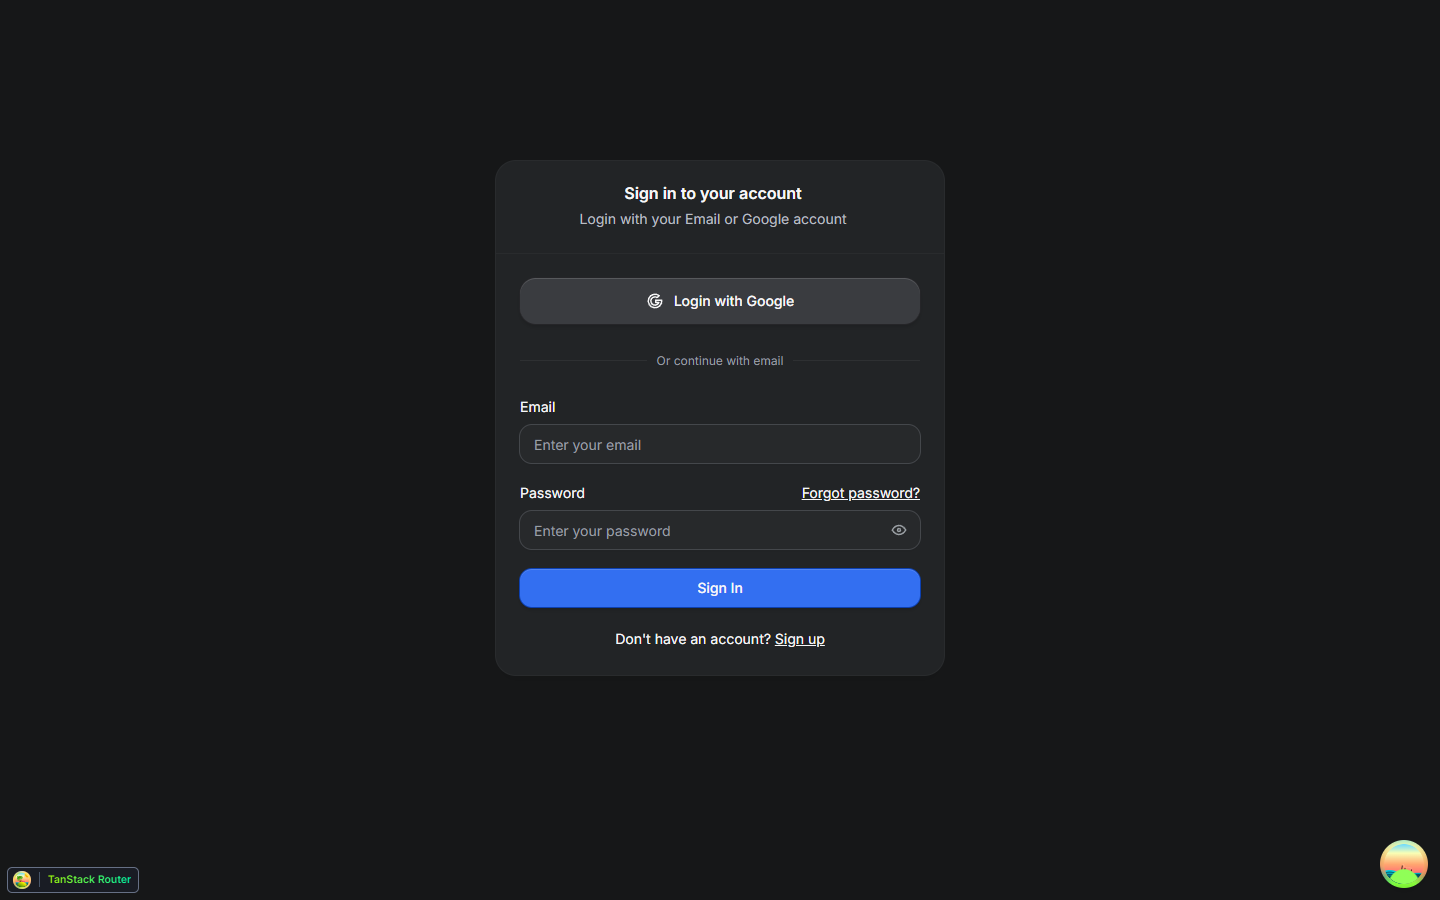
\includegraphics[width=0.7\textwidth]{01-login.png}
\end{center}

\subsection*{2. Halaman Sign Up}
\textbf{Route:} /login (toggle) \\
\textbf{Status:} Selesai

\begin{itemize}
    \item Field: Name, Email, Password
    \item Toggle show/hide password
    \item Validasi form
\end{itemize}

\begin{center}
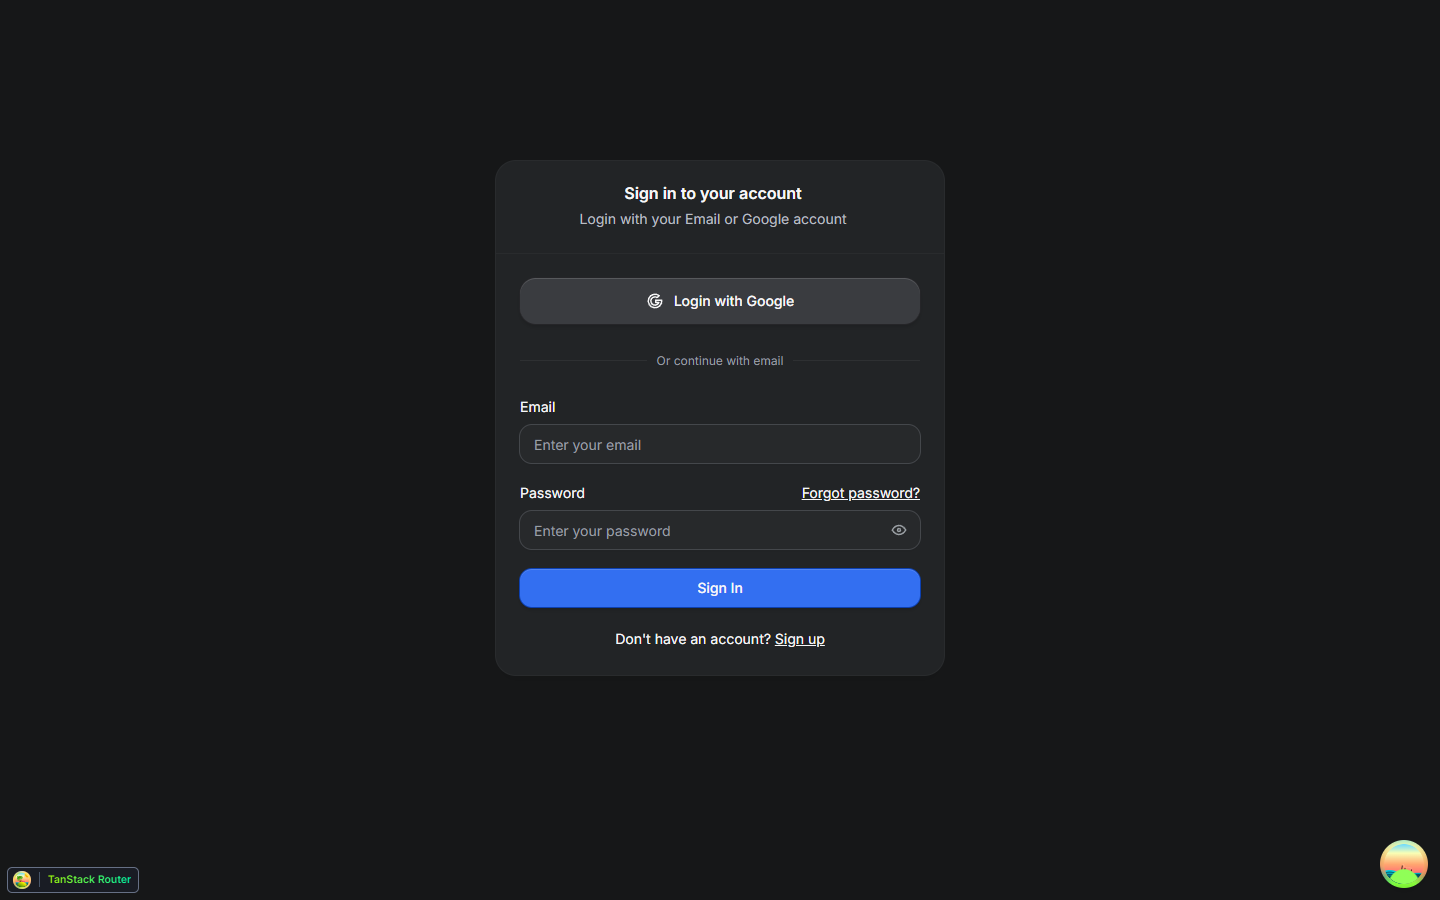
\includegraphics[width=0.7\textwidth]{01-login.png}
\end{center}

\subsection*{3. Dashboard}
\textbf{Route:} /dashboard \\
\textbf{Status:} \textcolor{orange}{Perlu Data Real}

\begin{itemize}
    \item Sidebar kiri dengan logo "Cogito" + search bar
    \item Navbar: judul, Notification Bell, Theme Toggle
    \item 4 Stat Cards (data masih dummy)
    \item "Best Selling" section (data masih dummy)
    \item User menu di footer sidebar
\end{itemize}

\textcolor{red}{\textbf{Catatan:}} Data dashboard masih menggunakan data contoh/template. Perlu diganti dengan data Cogito asli.

\begin{center}
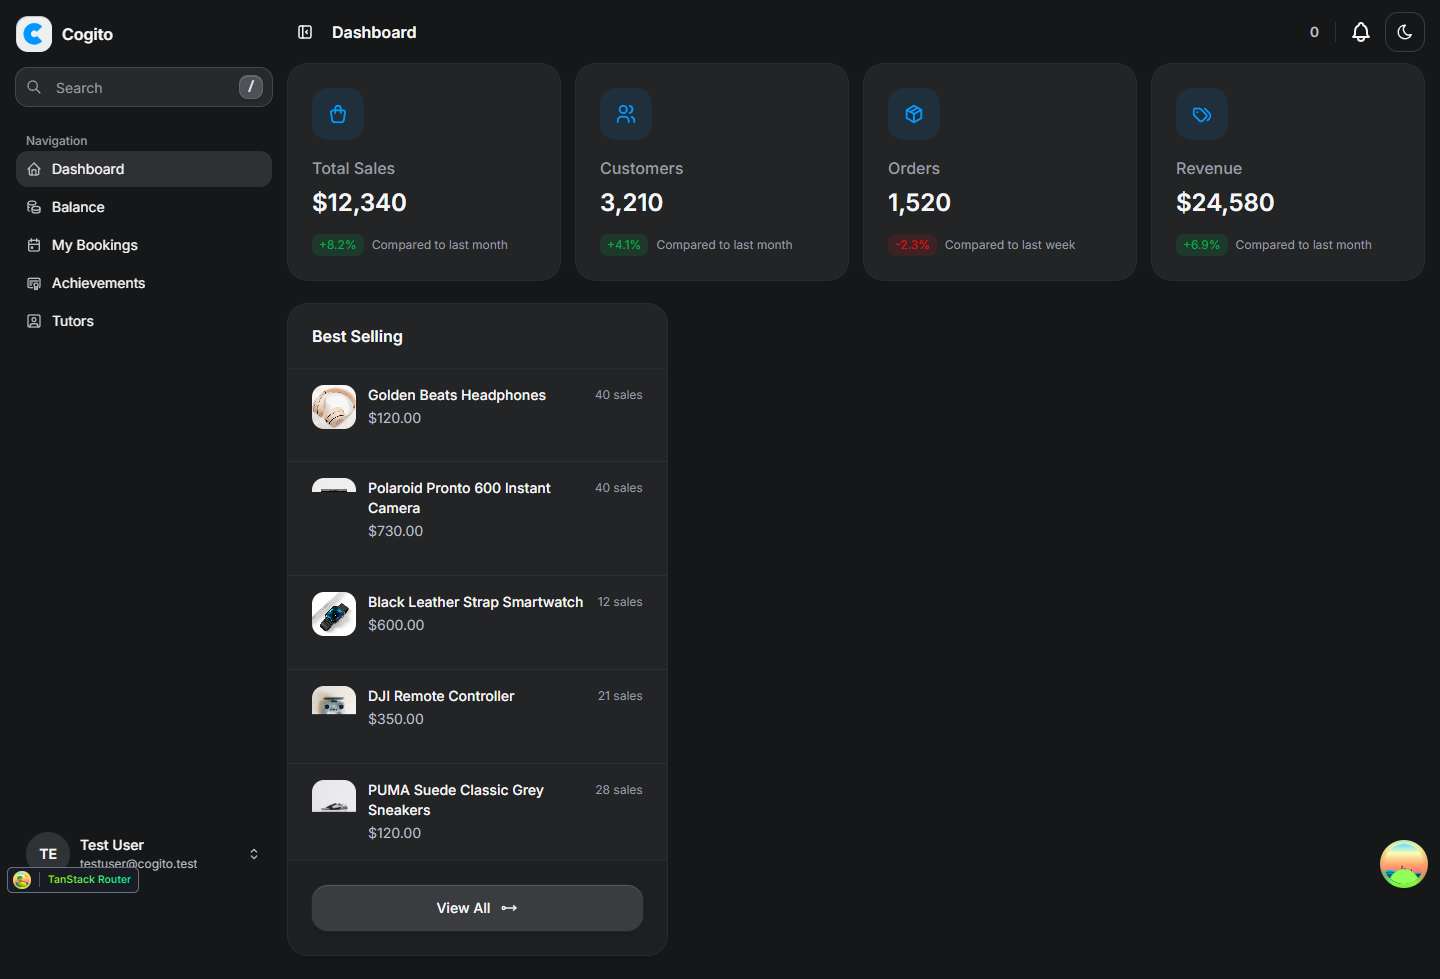
\includegraphics[width=\textwidth]{02-dashboard.png}
\end{center}

\subsection*{4. Halaman Saldo (Balance / Marks)}
\textbf{Route:} /balance \\
\textbf{Status:} Selesai

\begin{itemize}
    \item Total Balance, Held Balance, Available Balance
    \item Knowledge Bank Access (butuh minimal 35 Marks)
    \item Top Up Marks: 4 package (Pioneer, Explorer, Learner, Starter)
    \item Test mode active notice
\end{itemize}

\begin{center}
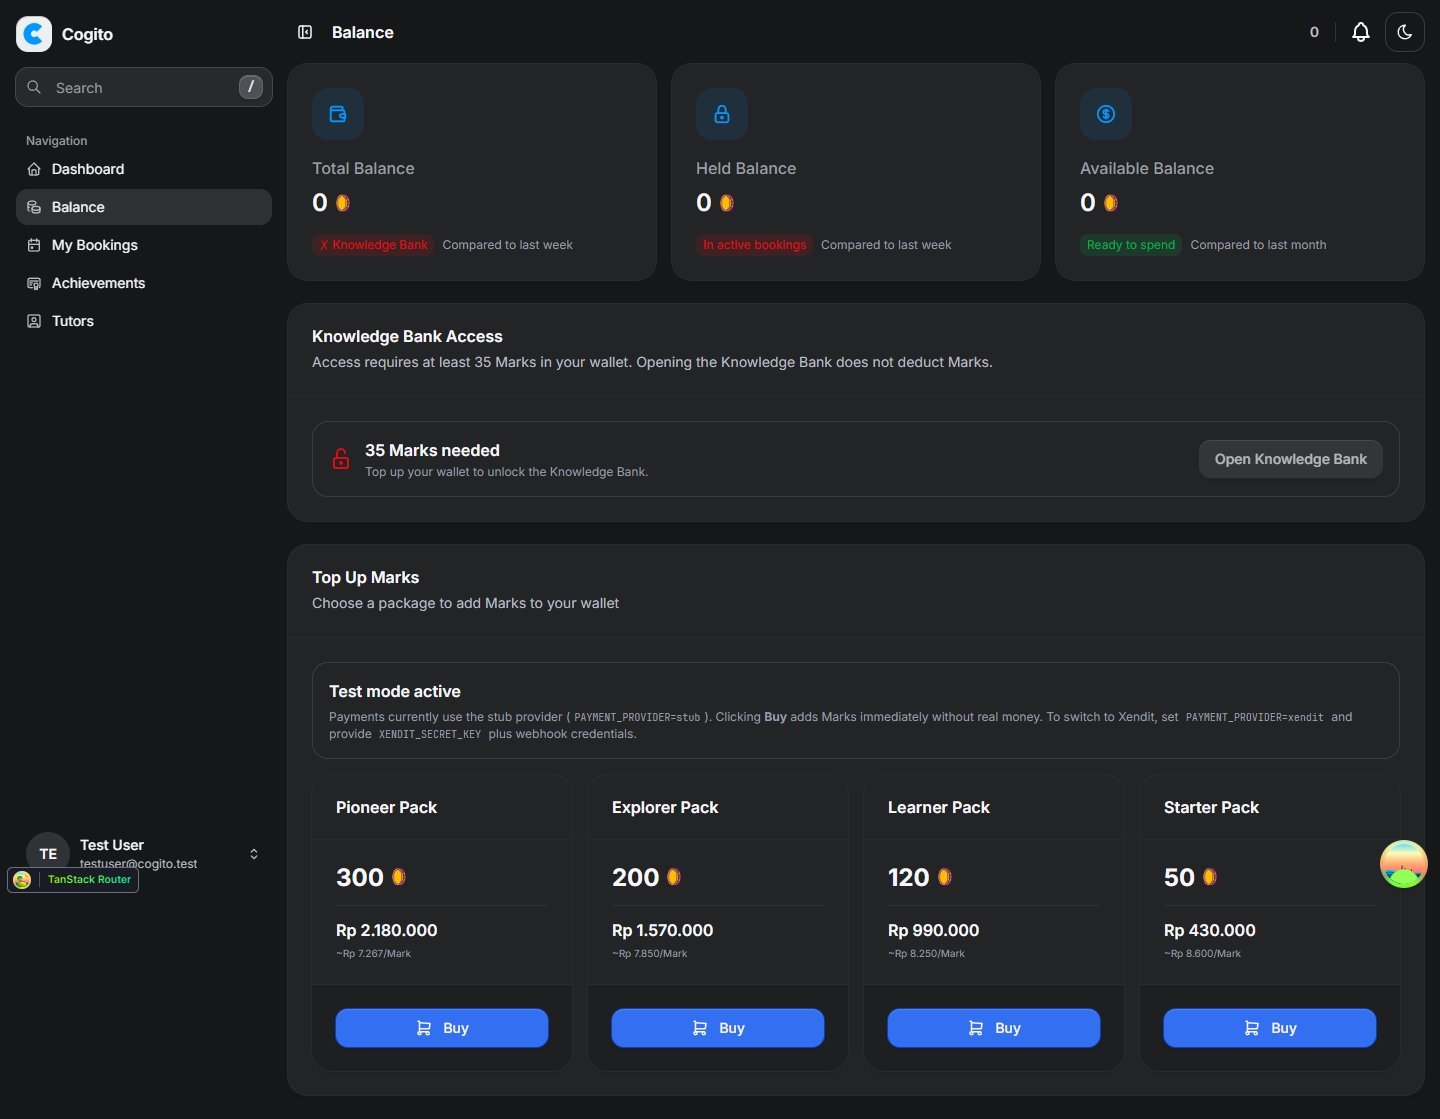
\includegraphics[width=\textwidth]{03-balance.png}
\end{center}

\subsection*{5. Halaman Booking Saya}
\textbf{Route:} /bookings \\
\textbf{Status:} Selesai

\begin{itemize}
    \item List booking dengan status badge (berwarna)
    \item Status: Awaiting tutor, Scheduled, Completed, Cancelled, Declined, Expired
    \item Tombol Cancel
    \item Empty state: "No bookings yet."
\end{itemize}

\begin{center}
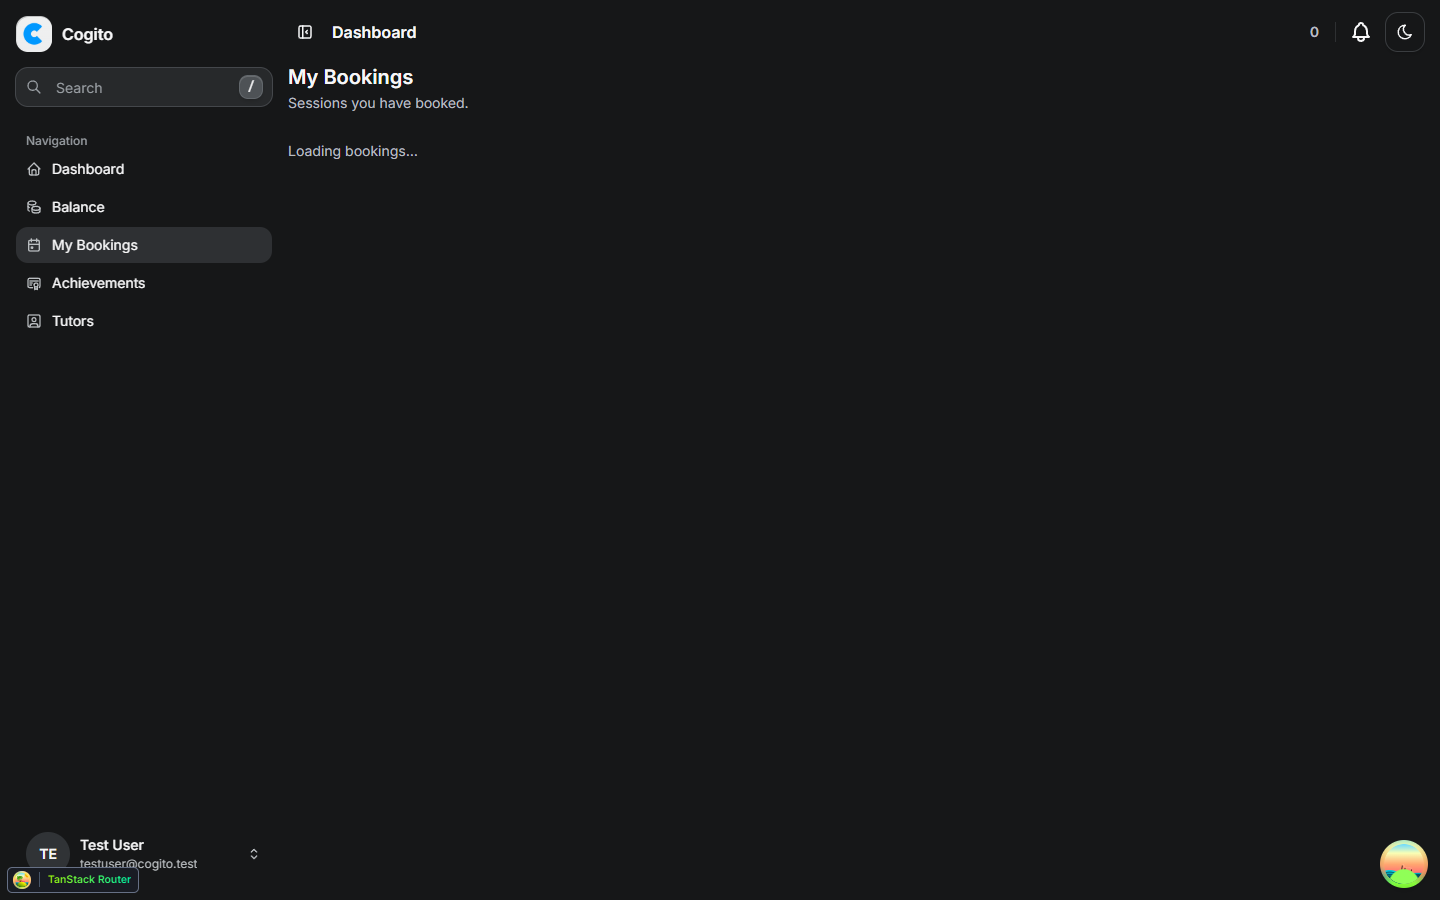
\includegraphics[width=\textwidth]{04-bookings.png}
\end{center}

\subsection*{6. Halaman Achievements}
\textbf{Route:} /achievements \\
\textbf{Status:} Selesai

\begin{itemize}
    \item Tambah Achievement
    \item Filter kategori \& status
    \item Stats: Total, Approved, Pending
    \item Empty state: "No achievements yet."
\end{itemize}

\begin{center}
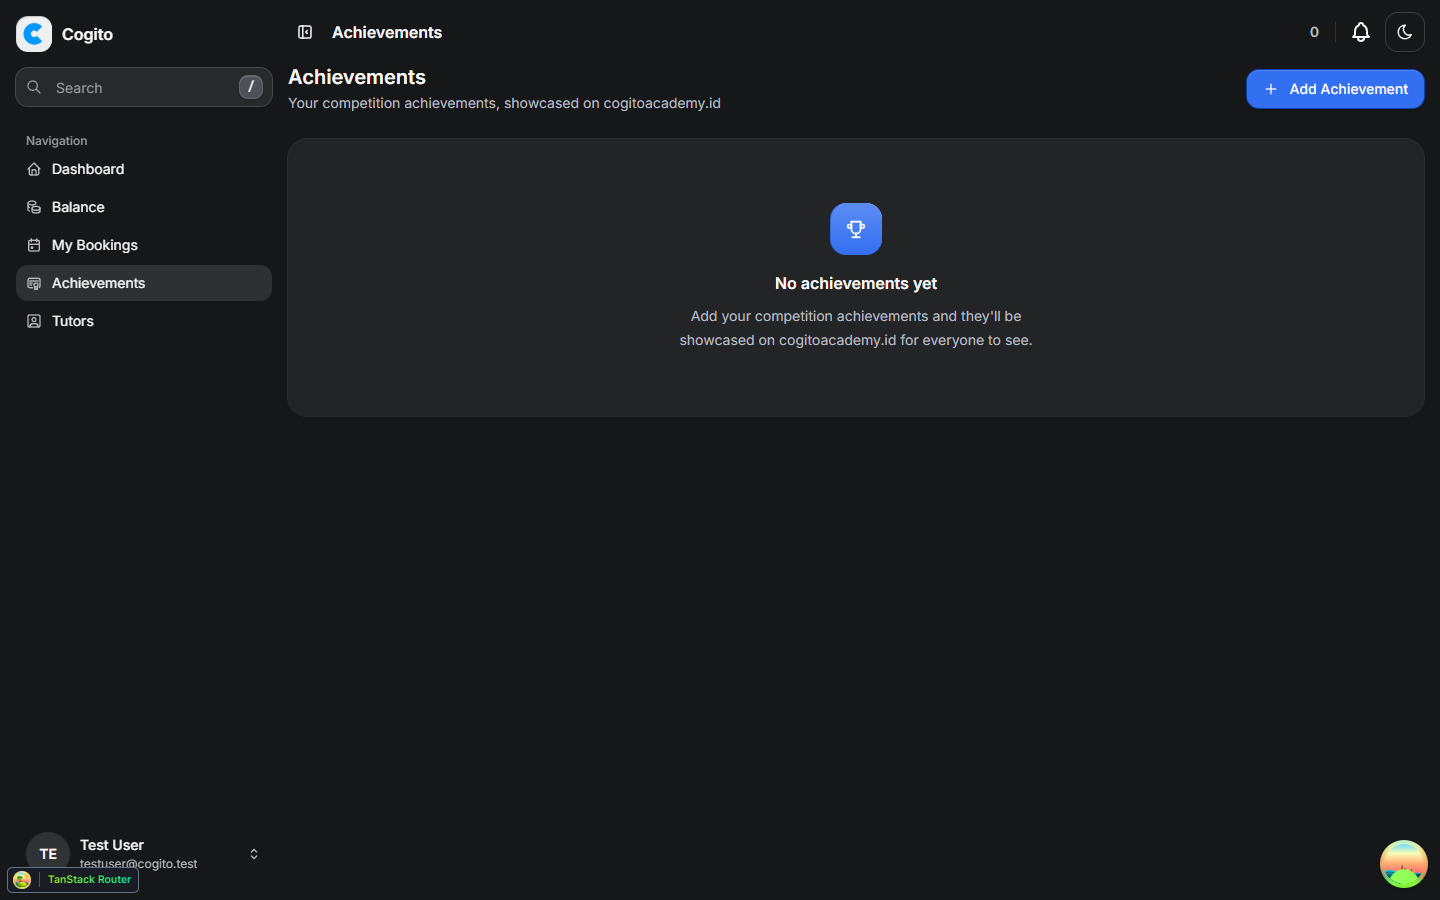
\includegraphics[width=\textwidth]{05-achievements.png}
\end{center}

\subsection*{7. Halaman Cari Tutor}
\textbf{Route:} /tutors \\
\textbf{Status:} Selesai

\begin{itemize}
    \item Search bar
    \item Filter Expertise (Mathematics, Physics, dll)
    \item Filter Modality (Online, Offline, Both)
    \item Grid card tutor dengan foto, nama, bio, badge
    \item Drawer detail tutor (slide-in)
    \item Loading skeleton
\end{itemize}

\begin{center}
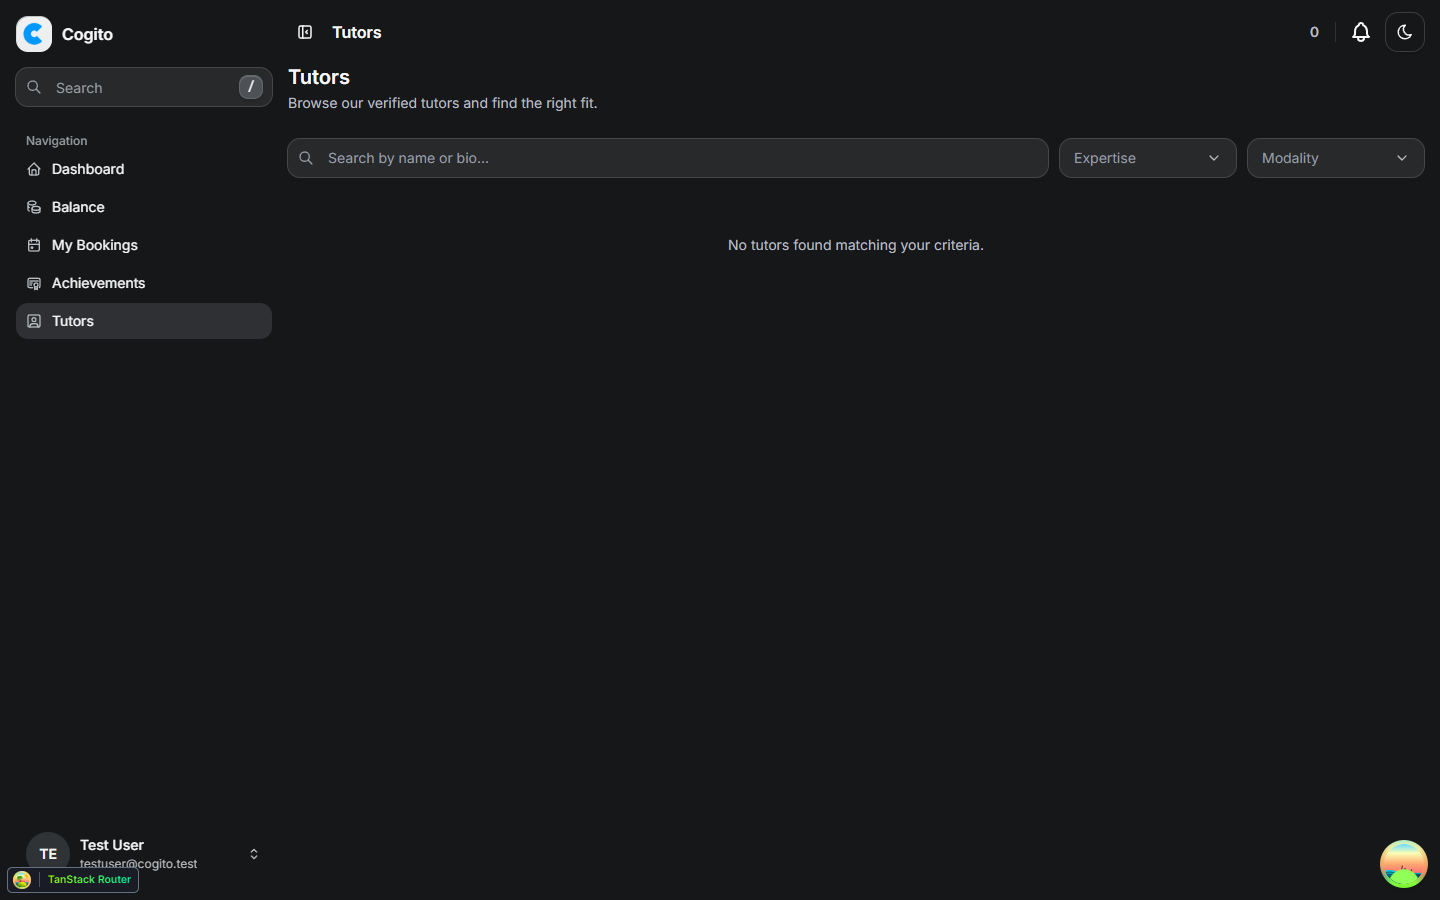
\includegraphics[width=\textwidth]{06-tutors.png}
\end{center}

\subsection*{8. Halaman Profile}
\textbf{Route:} /profile \\
\textbf{Status:} Selesai

\begin{itemize}
    \item Edit profil
    \item Field: Name, Email
    \item Tombol save
\end{itemize}

\begin{center}
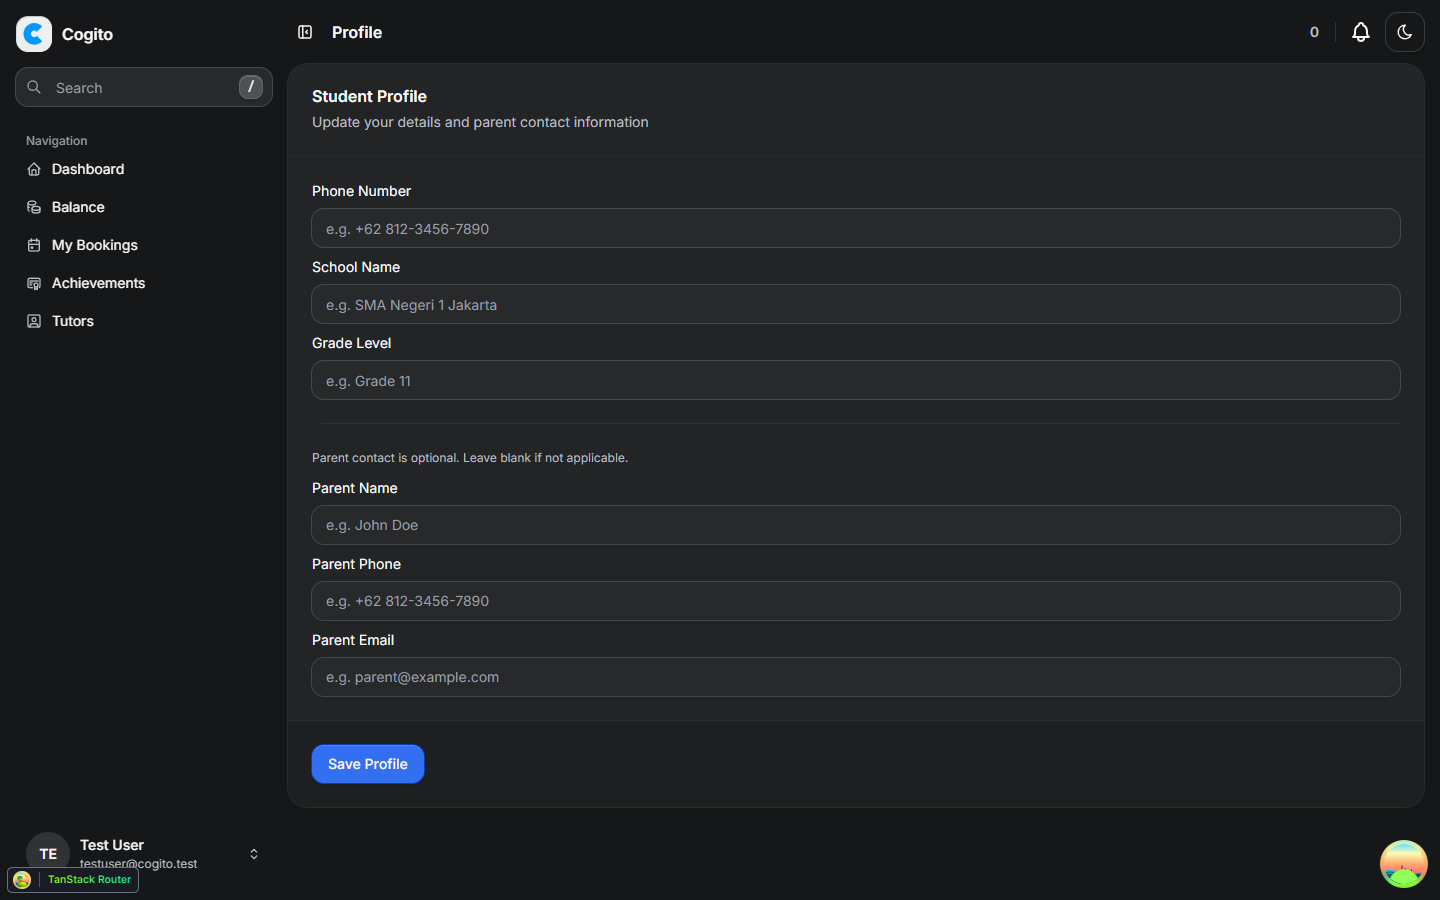
\includegraphics[width=0.7\textwidth]{07-profile.png}
\end{center}

\section*{Halaman Lainnya (Tidak Disertai Screenshot)}

\begin{enumerate}
    \item \textbf{Admin -- Kelola Tutor} (/admin-tutors) -- Selesai. Invite, review, approve tutor.
    \item \textbf{Onboarding Tutor} (/onboarding) -- Selesai. Form profil tutor.
    \item \textbf{Tutor Bookings} (/tutor-bookings) -- Selesai. Accept/Decline/Complete.
    \item \textbf{Notifikasi} (navbar) -- Selesai. Bell icon + dropdown.
    \item \textbf{Sidebar} -- Selesai. 3 role berbeda (Student/Tutor/Admin).
    \item \textbf{Invite Tutor} (/invite) -- Selesai. Claim undangan via token.
\end{enumerate}

\section*{Ringkasan Status}

\begin{center}
\begin{longtable}{|L{5cm}|c|L{5cm}|}
\hline
\textbf{Halaman} & \textbf{Status} & \textbf{Catatan} \\
\hline
Login & Selesai & Google OAuth + email \\
Sign Up & Selesai & Name, email, password \\
Dashboard & \textcolor{orange}{Perbaikan} & Data masih dummy \\
Balance / Marks & Selesai & Top up, Knowledge Bank \\
My Bookings & Selesai & List + cancel \\
Achievements & Selesai & Add, filter, delete \\
Cari Tutor & Selesai & Filter expertise \& modality \\
Profile & Selesai & Edit profil \\
Admin -- Kelola Tutor & Selesai & Invite, review, approve \\
Onboarding Tutor & Selesai & Form profil tutor \\
Tutor Bookings & Selesai & Accept/Decline/Complete \\
Notifikasi & Selesai & Bell icon + dropdown \\
Sidebar & Selesai & 3 role berbeda \\
Invite Link & Selesai & Claim via token \\
\hline
\end{longtable}
\end{center}

\vspace{1em}

\section*{Rencana Selanjutnya}

Berdasarkan \texttt{CONTEXT.md} dan rencana yang sudah ada di \texttt{docs/plans/}:

\subsection*{1. Consolidation (Improvement)}
\begin{itemize}
    \item Menyelesaikan arsitektur 4-layer di semua modul
    \item Migrasi driver database dari \texttt{pg} ke \texttt{postgres.js}
    \item Penerapan domain error architecture
\end{itemize}

\subsection*{2. Production Readiness}
\begin{itemize}
    \item Redis untuk session, idempotency, rate limiting, circuit breaker
    \item BullMQ scheduler untuk booking expiry, hold release, email dispatch
    \item Health check endpoint (\texttt{GET /health}) dengan DB + Redis ping
    \item Coverage threshold 80\% overall, 90\% untuk \texttt{packages/api}
    \item CD pipeline: build $\rightarrow$ push ke GHCR $\rightarrow$ migrate $\rightarrow$ deploy ke Coolify
\end{itemize}

\subsection*{3. Infrastructure}
\begin{itemize}
    \item Setup production deployment
    \item Docker containerization
    \item Environment configuration untuk production
\end{itemize}

\subsection*{4. PRD Gaps}
\begin{itemize}
    \item Mengecek dan menutup celah fitur terhadap Product Requirements Document
\end{itemize}

\subsection*{5. Bug Fixes (Prioritas Tinggi)}
\begin{itemize}
    \item \textbf{P0:} Meeting creation failure leaves booking in scheduled
    \item \textbf{P0:} Refund correction stores bookingId as paymentId
    \item \textbf{P0:} Series bookings never expire (no deadlineAt)
    \item \textbf{P0:} No CSRF protection on mutations
    \item \textbf{P1:} Triple session validation per request
    \item \textbf{P1:} Scheduler issues (onReleaseHolds, onSendNotificationEmail, graceful shutdown)
    \item \textbf{P1:} Refund createCorrection uses Date.now() in event key
    \item \textbf{P1:} applyOverride doesn't update booking.holdAmount
\end{itemize}

\subsection*{6. Data Dashboard Real}
Dashboard masih menampilkan data dummy. Perlu diganti dengan data Cogito asli.

\vfill

\begin{center}
\textit{Dokumen dibuat dari screenshot langsung aplikasi pada 23 Juli 2026.}
\end{center}

\end{document}
